\documentclass[10pt]{article}
\usepackage{amsfonts}
\usepackage{fancyhdr}
\usepackage{comment}
\usepackage[letterpaper, top=2.5cm, bottom=2.5cm, left=2.2cm, right=2.2cm]%
{geometry}
\usepackage{amsmath}
\usepackage{mathtools}
\usepackage{changepage}
\usepackage{enumitem}
\usepackage{amssymb}
\usepackage{graphicx}
\usepackage{hyperref}
\usepackage{listings}
\usepackage{color}
\usepackage{textcomp}
\usepackage{courier}
\definecolor{listinggray}{gray}{0.9}
\definecolor{lbcolor}{rgb}{0.96,0.96,0.96}
\lstset{
    backgroundcolor=\color{lbcolor},
    tabsize=4,
    rulecolor=,
    language=Python,
        basicstyle=\footnotesize\ttfamily,
        upquote=true,
        aboveskip={1.0\baselineskip},
        columns=fixed,
        extendedchars=true,
        breaklines=true,
        prebreak = \raisebox{0ex}[0ex][0ex]{\ensuremath{\hookleftarrow}},
        frame=single,
        showtabs=false,
        showspaces=false,
        showstringspaces=false,
        identifierstyle=\ttfamily,
        keywordstyle=\color[rgb]{0,0,1},
        commentstyle=\color[rgb]{0.133,0.545,0.133},
        stringstyle=\color[rgb]{0.627,0.126,0.941},
}

\newcommand{\by}{\mathbf{y}}
\newcommand{\vertdots}{\underset{\big{\overset{\cdot}{\cdot}}}{\cdot}} 
\newcommand{\diagdots}{_{^{\big\cdot}\cdot _{\big\cdot}}}

\begin{document}

    \title{SDS 383D, Exercises 2: Bayes and the Gaussian Linear Model}
    \author{Tyler Buffington}
    \date{\today}
    \maketitle

    \section*{Bayseian linear model}
    The code for the Bayesian linear model is in the file bayeslinmodel.py. It's derivation is detailed in mathnotes.pdf. The main takeaway from the results is that the fit is very sensitive to the choice of the prior precision matrix. If we choose the matrix $\begin{bmatrix} 0.1 & 0 \\ 0 & 0.1 \end{bmatrix}$, we get the fit shown below:

     \begin{figure}[htb] \centering
         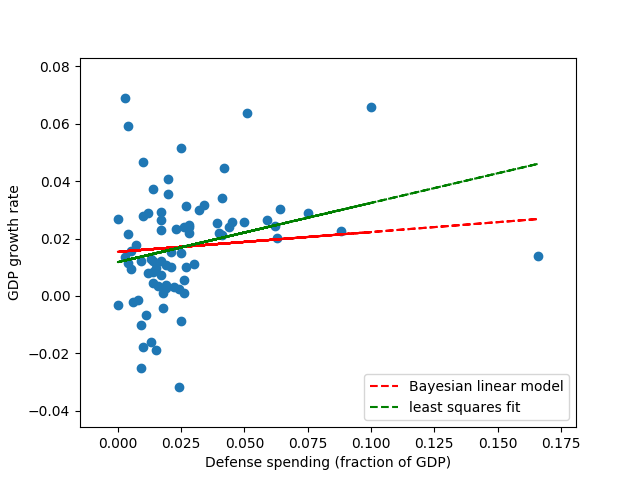
\includegraphics[width=0.95\textwidth]{./linear_bayes_prior.png}
         \caption{The fit for a specified K matrix}
         \label{fig:bayes_wprior}
     \end{figure}

    Note that the Bayesian linear model result is between the OLS estimate and the prior estimate, which is a flat line at y=0.

    If we do not choose a prior, the code will by default assign a diagonal K matrix with values of $10^{-12}$. This gives a result that converges to the OLS estimate. We can see below that the least squares fit and the Bayseian linear model result are on top of each other.

     \begin{figure}[htb] \centering
         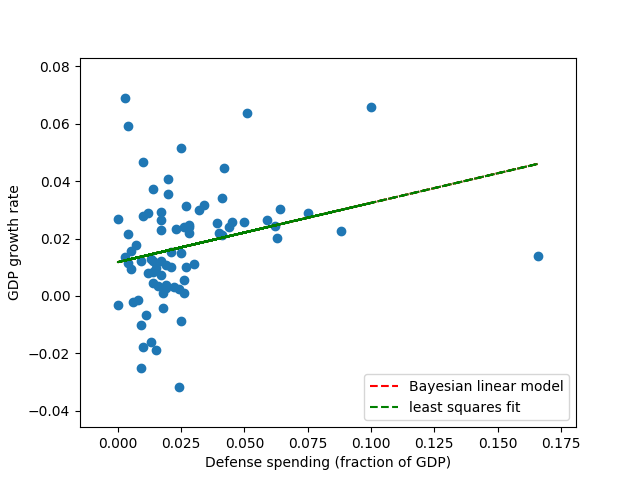
\includegraphics[width=0.95\textwidth]{./linear_bayes.png}
         \caption{The fit for no specified K matrix}
         \label{fig:bayes_no_prior}
     \end{figure}
     \section*{Heavy tailed model}
     The code for the Gibbs sampler is in the file heavy\_tailed.py. The resulting fit is shown below:

     \begin{figure}[htb] \centering
         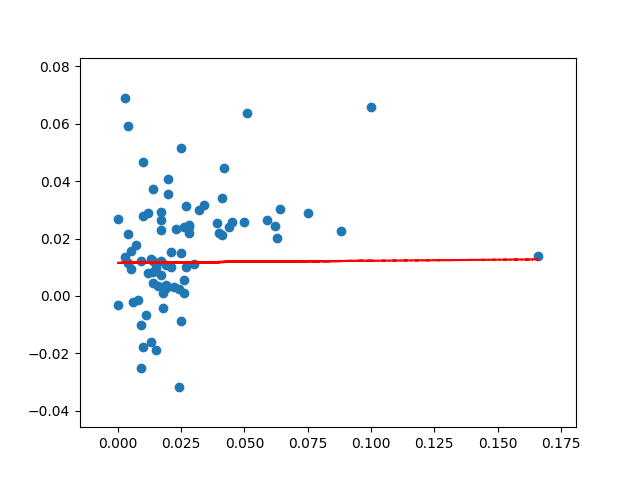
\includegraphics[width=0.95\textwidth]{./heavy_tail_fit.png}
         \caption{The fit from the heavy tailed model}
         \label{fig:heavy_fit}
     \end{figure}
\end{document}
